%!TEX root = ../vernier.tex
\section{Projection} \label{sec:proj}
Multidimensional projections (MP) are a set of techniques that allow efficient and effective visual analysis of high-dimensional data. They do so by mapping data points from a high-dimensionality space ${\mathbb{R}^{n}}$ to a low-dimensionality space $\mathbb{R}^{m}$, where ${n > m}$ and ${m \in \{2,3\}}$. This mapping aims to preserve the neighborhoods present in  ${\mathbb{R}^{n}}$, generating visual representations that naturally convey the similarity relationship present in the data points.

When compared to other high-dimensional visualization techniques such as table lenses \cite{ref:solid}, evolution lines \cite{ref:evolines}, evolution matrices \cite{ref:evomat}, parallel coordinates \cite{ref:parallelcoords}, and scatterplot matrices \cite{ref:scatter}, multidimensional projections are considerably more scalable in number of entities and dimensions it can handle, it is also specially easy to find groups of related entities.

Modern MP techniques, such as ISOMAP \cite{ref:tenenbaum2000ISOMAP}, LAMP \cite{joia2011LAMP}, LSP \cite{paulovich2008LSP}, and t-SNE \cite{maaten2008tsne} score highly in distance preservation for static datasets, however, none of them is able to handle time-dependent datasets. The recent dynamic t-SNE (dt-SNE) \cite{ref:dtsne} technique is, to our knowledge, the only MP for time-dependent datasets that offers explicit and verified guarantees in terms of spatial and temporal coherence. Trade-off between preservation of distances in the same projection $vs$ preservation of distances across projections which are close in time is controlled by a user parameter.

Figure \ref{fig:dtsne} illustrates on the left how the original t-SNE technique doesn't take into consideration the previous position of a group of entities and might place it in a distant locale, whilst the dt-SNE technique on the right tries to preserve the previous neighborhood layout.
\begin{figure}[H]
  \centering
  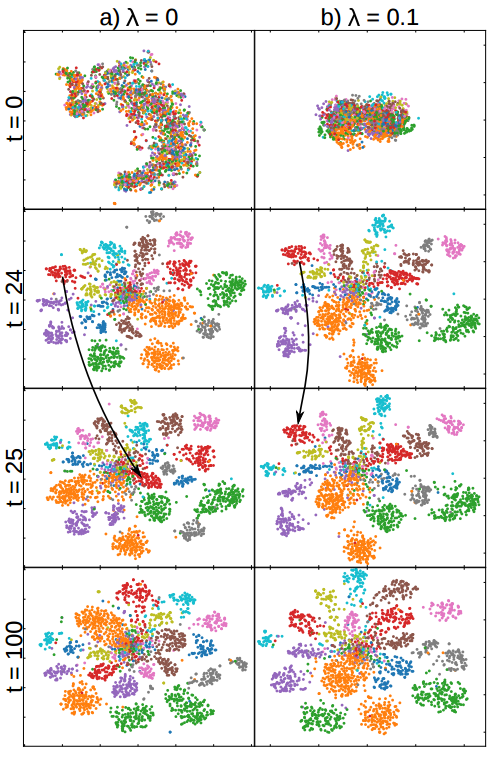
\includegraphics[width=0.6\textwidth]{figures/dtsne.png}
  \caption{Dynamic t-SNE results on SVHN CNN}
  \label{fig:dtsne}
  \legend{Source: \cite{ref:dtsne}}
\end{figure}

Projections serve two main goals. First, by simply removing a number of dimensions that are highly correlated or present low variance, we are able to create a simpler and easier to handle representation of the original dataset that might suit our needs. Secondly, projections can be used to assist in the exploration on high-dimensionality datasets. In this case, instead of eliminating a number of dimensions, all attributes are taken into consideration on the ${\mathbb{R}^{n}}$ to ${\mathbb{R}^{m}}$ mapping, generating a visual representation that can be conceptually understood in the same fashion as a 2D scatterplot or a 3D point could.

In our approach, for each revision $r_{t}$ $\in$ $[r_{s}, r_{e}]$, dt-SNE is used to generate a 2D projection $P_{t} = \{q_{i} \} \subset{\mathbb{R}^{2}}$ such that the pairwise distance between points $\Vert q_{i} - q_{j} \Vert$ are as close as possible to the high-dimensional space distance $\Vert e_{i} - e_{j} \Vert$ and the distances between the same point in consecutive revisions $E_{t1}$ and $E_{t2}$ are preserved.
